\chapter{Read-Optimized Databases}
\label{chap:olap}
This chapter forms the background theory on databases that are optimized for analytical workloads, where the main motivation is to investigate which technologies enable high performance data processing to accomodate such workloads. The chapter elaborates on storage formats, compression, and testing, and also background theory on modern CPUs.\todo{rewrite when chapter done} We emphasize techniques used in in-memory databases, although most of our findings apply to disk-based databases as well.

The sources used to form this chapter were found using the \textit{Snowballing} method. During this research, we identified several database systems and \bi~solutions which apply the various techniques. \todo{Not sure if this is specific enough}

\todo{For chapter: Ask bratsberg and genus whether content is too much, too little? Needs språkvask}

\clearpage

\section{Database Terminology}
\label{sec:Database Terminology}
This section presents terms and definitions central in the database field and is important to understand the contents of this chapter.

\paragraph{Online Analytical Processing (OLAP)}
\label{par:Online Analytical Processing (OLAP)}
  We use the term Online Analytical Processing (OLAP) extensively in this chapter. By OLAP, we mean systems that enable users to analyze multidimensional data interactively from multiple perspectives \cite{Wikipedia_contributors2015-hw}. OLAP is usually dominated by ad-hoc, complex queries that group, aggregate and summarize over large datasets \cite{Bjorklund2011-wh}. OLAP systems can be both disk and memory-based. Column storage is considered to be an attractive solution for OLAP systems, a technique we study further in Section \ref{sec:Column Storage}.


\paragraph{Online Transactional Processing (OLTP)}
\label{par:Online Transactional Processing (OLTP)}
Online Transactional Processing (OLTP) is a class of database systems that manage transaction-oriented applications \cite{Wikipedia_contributors2015-cw}. Transactional workloads are typically referred to as insertion of new records, as well as updates and deletes of single records in the database. An OLTP system normally uses row storage for its data.

\paragraph{Database Management System (DBMS)}
\label{par:Database Management System (DBMS)}
A Database Management System (DBMS) is a computer software application for storage and analysis of data \cite{Wikipedia_contributors2015-pb}. The most common way to interface with a database is through SQL, although other methods exist. Regarding performance, DBMSes can focus on analytical workloads (OLAP), transactional performance (OLTP), or both. In this literature review, we look at several systems, including \oracle, \ibm, \saph, \sapnw, \mssql, \cstore, \vertica, \blink, \exasol, \oracle, \hyper, and \hyrise. \todo{shorten this list?}

\paragraph{Business Discovery}
\label{par:Business Discovery}
\bd~is a term introduced by a \textit{QlikView} whitepaper \cite{Qlik2014-vd}. \bd~products differ from traditional \bi~systems by focusing more on the end user. \bd~products do not rely on aggregated data such that the user can follow his "information scent" and click his way through the data. \bd~platforms often provide an architecture that enables panels and dashboards to be shared with multiple clients, both on desktops and mobile devices. Current \bd~products typically build on tailored storage systems that are specifically designed for \bd~workloads, but some of them integrate directly with read-optimized DBMSes. \bd~products include \tableau, \qlikview, \powerpivot, and more. \bd~is explained in greater detail is Section~\ref{sec:Business Discovery}. \todo{Explain why bd is relevant?}


\section{Column Storage}
\label{sec:Column Storage}

\begin{figure}
  \centering
  \begin{subfigure}{\textwidth}
    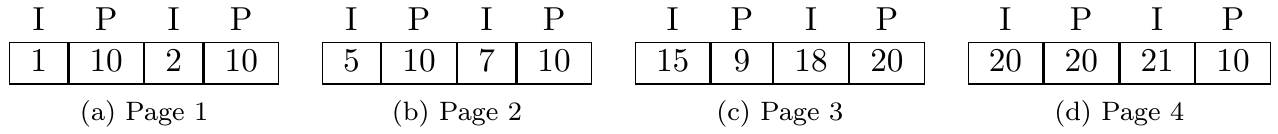
\includegraphics[width=\textwidth]{img/row-store.png}
    \caption{Row store layout.}
    \label{fig:row-column-store-1} 
  \end{subfigure}
  \begin{subfigure}{\textwidth}
    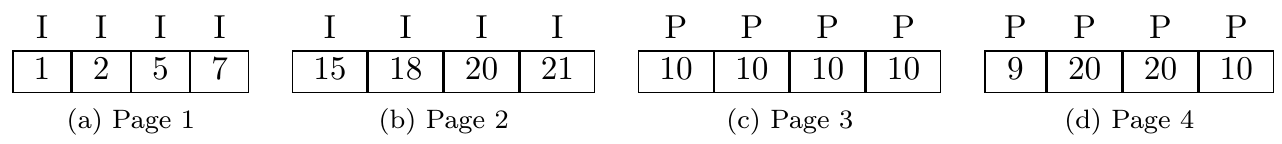
\includegraphics[width=\textwidth]{img/column-store.png}
    \caption{Column store layout.}
    \label{fig:row-column-store-2} 
  \end{subfigure}
  \caption{Row and column oriented layouts for a table with two columns, I and P. In the row-oriented layout (a), records (I and P tuples) are stored next to each other within the pages. In the column-oriented layout (b), values from the I column and P column are stored separately on different pages. (Adapted from \cite{Bjorklund2011-wh})}
  \label{fig:row-column-store} 
\end{figure}

The most common storage format for OLTP systems is row storage, as we briefly mentioned in Section \ref{sec:Database Terminology}. Row storage enables easy fetching of values from the same tuple and is suited for updates, inserts, and deletes. However for OLAP workloads, columnar storage has turned out advantageous, mainly because of two reasons: First, aggregations are easier, since calculations are performed on data consecutive in memory. Second, column storage does not fetch more data than is needed for the query.

Our research has identified several systems using columnar storage. These include \monetdb~\cite{Boncz2005-wj, Boncz2002-yj}, \cstore~\cite{Stonebraker2005-qz}, \saph~\cite{Farber2012-vh}, and \mssql~\cite{noauthor_undated-vq, Larson2013-mc}, as well as the \bd~product \tableau~\cite{Kamkolkar2015-iq}.

In a column store, each column in a table is stored separately in a continuous segment (unless data is horizontally partitioned, see Section \ref{sub:Horizontal Partitioning}), as opposed to row stores where attributes from a single row are stored together \cite{Bjorklund2011-wh}. Figure \ref{fig:row-column-store} depicts both row and column oriented layouts for a table with two columns (I and P). The row storage alternates between I and P to store records next to each other on the pages while the column storage keeps I and P values separate. 

The advantages of using column storage are many. The primary one is that no more data is accessed than strictly necessary for a query. In addition to this, columns are inherently more compressible \cite{noauthor_undated-vq}. Compression leads to higher performance due to better cache and memory utilization, and this effect is one of the reasons why \mssql~use column storage. We elaborate on the performance benefits of compression in Section \ref{sec:Compression}.

Column storage also comes with a more subtle advantage; columns have a \textit{low degree of freedom} compared to row storage \cite{Boncz2005-wj}. When operating on column values, only the local memory offset is required, not the global table layout. This removes some layers of indirection and query processing can be made more efficient. Boncz \ea~claim that this is the main reason why column storage is advantageous.

One of the major disadvantages with column store is that it is not as easily updateable \cite{Bjorklund2011-wh}, especially if the columns are compressed or sorted. This challenge is typically overcome using a separate structure for writes and updates called a \textit{delta store}. Using such structure, the main part of the database is stored column-wise in a static structure optimized for reads while the updates and inserts are accumulated in a smaller and more dynamic structure. \todo{Consider ditching this paragraph entirely} 

Another disadvantage with column storage is tuple materialization costs. Since the result of most DBMS queries should be returned as rows, columns must be stitched back together before returned to the client, an operation that can be expensive.

\subsection{Sorting}
\label{sub:Sorting}
Few systems sort values within a column, with the exception of \cstore~\cite{Stonebraker2005-qz} and \vertica~\cite{Lamb2012-kg}. Sorting values in a column store comes with some advantages. First, single value lookups are easily performed by a binary search. Second, and perhaps most important, is that sorted columns can be compressed aggressively by applying \rle. \rle~is the main reason \cstore~stores sorted data. We study this type of compression in Section \ref{sec:Run-Length Encoding}.

Except from \cstore~and \vertica, our research has shown little indication that sorting values in columns are common. For instance, \mssql~\cite{Larson2013-mc}, \blink~\cite{Raman2013-em} and \oracle~\cite{Lahiri2015-mz} accept values in the order they appear.

Although most systems do not sort values in the columns and instead accept values as they arrive, many systems have a sorted dictionary when \de~is used. Systems here include \blink~\cite{Johnson2008-cp} and \saph~\cite{Farber2012-vh}. A sorted dictionary has many advantages, like an easy lookup for single values, transformation of range predicates to \texttt{IN}-list predicates, and partition pruning. A sorted dictionary structure is better suited for a read-only environment since updating a sorted dictionary requires some work. We look into \de~in Section \ref{sec:Dictionary Encoding}. \todo{Ditch this paragraph?}

\subsection{Row Stores vs Column Stores}
\label{sub:Row Stores vs Column Stores}
Most research agrees that row stores are most suitable for OLTP workloads, and column stores are most suitable for OLAP workloads. Abadi \ea~set out to investigate whether there is a fundamental difference between row and column stores \cite{Abadi2008-dd}. In their research, they used a row store with a vertically partitioned schema to mimic a column store. They also tried applying indexes to each column such that each column could be accessed independently. Their conclusion was that there \textit{is something fundamental about column stores} that makes them perform so well, and that changes must be done to both storage layer and query executor to obtain the benefits of a column-oriented approach. The main reasons why column storage is better suited for OLAP workloads are:
\begin{itemize}
  \item \textit{Compression}, which we discuss in Section \ref{sec:Compression}.
  \item \textit{Vectorized execution}, which we discuss in Section \ref{sec:Loop Pipelining and Vectorized Execution}. 
  \item \textit{Late materialization}, which we discuss in Section \ref{sub:Late Materialization}. 
\end{itemize}

There are situations for OLAP databases where a row store performs better than a column store. A research executed by Holloway \ea~shows that a row store can outperform a column store when processing time is the dominating constraint \cite{Holloway2008-rr}. This is typically the case for low selectivity queries and queries with many predicates. To further improve row storage performance, tuples can be compressed. However, row storage will most likely never beat column stores for OLAP workloads, since bandwidth requirement for processing rows is higher than for columns.

We have also identified papers that claim OLTP databases also benefit from a columnar storage. The work of Farber \ea~argues that columnar storage is suited for transactional workloads as well, mainly due to the compression \cite{Farber2012-vh}. Also, storing data in columns allows for dropping indexes, which is normally costly to maintain. Last, there are usually a lot more read operations than inserts, updates, and deletes in an OLTP database.

\ffigure{img/chain-reaction.png}{OLTP workloads will affect more than a couple of rows. Index structures must be maintained, and aggregations and materialized views must be updated. In the figure, an update that triggers a chain reaction is depicted. (Adapted from \cite{Plattner2014-fr})}{fig:chain-reaction}
Plattner \ea~claim that most OLTP queries request aggregates instead of single rows \cite{Plattner2014-fr}. Also, updates to the database normally trigger a chain reaction of updates to indexes and materialized views, as seen in Figure \ref{fig:chain-reaction}. Their conclusion is that column storage is suited for OLTP databases due to efficient aggregation and absence of indexes. The absence of indexes also makes application development easier, since no performance layer must be specified by the application programmer. \todo{merge this with above paragraph?}

\subsection{Row Identifiers and Tuple Materialization}
\label{sub:Row Identifiers and Tuple Materialization}
A row in a column store is identified by a unique identifier that is common to every value belonging to the same row in a table. Many systems store these IDs implicitly as virtual object IDs (\texttt{void}). A \texttt{void} for an object is calculated using a base ID and the offset from the first value in the column. For instance, the fourth value of a column with base ID 100 has an implicit ID of 103. \texttt{void} type identifiers are used in \monetdb~\cite{Boncz2002-yj}, \cstore~\cite{Stonebraker2005-qz}, \vertica~\cite{Lamb2012-kg}, and \ibm~\cite{Raman2013-em}. Although stitching together rows in a column store is a trivial operation, it comes at a higher cost than in a row store. \todo{Link datasource index to this}

If horizontal partitioning is used, a technique we discuss in the next section, the partition number must also be accounted for in row identification. For instance, \mssql~identifies a row by a combination of row group ID and tuple ID \cite{Larson2013-mc}.

\subsection{Horizontal Partitioning}
\label{sub:Horizontal Partitioning}
Several systems split columns horizontally. Partitioning data horizontally can be beneficial due to the following reasons:
\begin{itemize}
  \item Storing metadata, like minimum and maximum values per block, exploits clustering in the data. A partition block can be skipped entirely if a predicate is outside the value range of a block.
  \item If each partition has its dictionary, the dictionary can be scanned for the presence of a key. If the key is not there, the partition can be skipped.
  \item Smart partitioning of data based on the value frequencies handles data skew and allows for improved compression rates \cite{Raman2008-gi}. 
  \item Partitions provide a logical division of data that can be processed simultaneously. The division enables parallelization and balance \cite{Exasol2014-xh}.
  \item Horizontal partitions can be created one at a time, such that new insertions will not affect already existing partitions. New data can be accumulated in temporary structures, and when there are enough rows in these structures, read-only column partitions can be created and inserted into the database.
  \item The operating system might not be able to provide memory chunks large enough to contain an entire column. Horizontally partitioning the data will help overcome this limitation.
\end{itemize}

\ffigure{img/mssql-row-group.png}{This figure illustrates how a column store index in \mssql~is created and stored. The set of rows is divided into row groups that are converted to column segments and dictionaries. (Adapted from \cite{Larson2013-mc})}{fig:mssql-row-group}

Instead of operating on entire columns at a time, \mssql~divides the data into \textit{row groups} that are groups of rows compressed into a columnar format \cite{Larson2013-mc}. Within the columns, data is not sorted. Each row group is encoded and compressed independently, and as we see in Figure~\ref{fig:mssql-row-group}, each partition has its own dictionary. We were unable to find out how many rows are contained by each row group, but the Larson \ea~say that the number of rows in a row group must be small enough to benefit from in-memory operations and large enough to achieve high compression rates. 

For \oracle, the column store is made up of multiple extents, called In-Memory Compression Units (IMCUs) \cite{Lahiri2015-mz}. Much like \mssql, data is loaded into the IMCUs without a sort order; they are stored the same way as they appear in the row format. Each partition consists of approximately half a million rows, and each IMCU contains maximum and minimum values per column such that data can be pruned easily. \todo{Merge with above?}

\section{Compression}
\label{sec:Compression}
Historically, compression has been thought of a measure for reducing disk usage and memory footprint. However, in our case, compression of data also comes with the benefit of increased performance. A study conducted by Abadi \ea~looked into database compression for in-memory databases, and concluded compression increases performance by a factor of two on average \cite{Abadi2008-dd}.

Among systems we have studied in this literature review, we have identified several that applies compression for performance reasons. Among these systems are \ibm~\cite{Raman2013-em}, \cstore~\cite{Stonebraker2005-qz}, \vertica~\cite{Lamb2012-kg}, \oracle~\cite{Oracle2015-fs}, \gorilla~\cite{Pelkonen2015-ko}, and \exasol~\cite{Exasol2014-xh}. In addition to this, \bd~products \tableau~and \qlikview~also use compression extensively to achieve good performance \cite{Kamkolkar2015-iq, Qlik2014-vd}. 

Compression of data in a database is beneficial for performance due to:
\begin{itemize}
  \item Cache locality is improved \cite{Exasol2014-xh}. More values from a single column (or record) fit in the cache at the same time.
  \item Memory traffic is reduced. Compression can help turning a database from memory-bound to CPU bound \cite{Willhalm2009-hu}.
  \item Compression reduce CPU cycles \cite{Stonebraker2005-qz}. First of all, as stated above, it reduces memory latency and improves cache locality, such that more cycles can be used for calculations and not waiting for memory. Besides, compression enables working on multiple values in parallel using SIMD instructions, as we see in Section \ref{sub:SIMD}.
\end{itemize}

Still, even though compression is used to increase database performance, the fact that compression reduces memory usage is also important. Even though DRAM is cheap, it is rarely over-provisioned and unused \cite{Barber2014-ey}. Also, compressed data frees up space for other structures, like indexes and result caches. For instance, \oracle~justifies their dual format by using the space freed up by compressing the columns \cite{Lahiri2015-mz, Lamb2012-kg}. Compression can help an application avoid relying on slow, virtual memory.

\subsection{Compression Types and Light-Weight Compression}
\label{sub:Compression Types and Light-Weight Compression}
A study performed by Westmann \ea~investigates database compression, and concludes that that the compression must be \textit{light-weight} for maximum performance \cite{Westmann2000-mz}. In other words, the real benefit of compression can only be leveraged if the decompression effort can be minimized \cite{Lemke2010-is}. Light-weight compression has been defined by Holloway \ea~as \bp, \de, \dele, and \rle~\cite{Holloway2008-rr}. Holloway \ea~also conclude that \de~and \rle~are the best compression schemes for column stores. These compression techniques are fast and fine-grained, which is important for performance.

Zukowski \ea~conclude that a compression algorithm should care about super-scalar processors. This implies that the algorithm should be able to pipeline loops, support out-of-order execution, and avoid if-then-else in inner loops \cite{Zukowski2006-oz}. We study modern CPUs and compilers in Section \ref{sec:Modern CPUs and Compilers}.

A database can use multiple compression schemes. First, most of the light-weight compression techniques can be combined, where the most common combination is \de~and \bp. We study this idea in Section \ref{sec:Dictionary Encoding}. Second, different compression schemes can be used for different columns. In Section \ref{sub:Sorting}, we saw that \cstore~and \vertica~allow for multiple column projections (a subset of the columns), where each projection is sorted based on one of the columns in the subset. 

\subsection{Working Directly on Compressed Data}
\label{sub:Working Directly on Compressed Data}

\afigure{img/ram-cache-decompression.png}{I/O-RAM vs RAM-CPU compression. In the left sub-figure, data is decompressed before it is put in the buffer manager (RAM). In the right sub-figure, data is kept compressed in the buffer manager and only decompressed when it is brought into the CPU cache. (Adapted from \cite{Zukowski2006-oz})}{fig:ram-cache-decompression}{0.8}

Earlier database systems with compression, data was decompressed when brought up to RAM. In 2006, Zukowski \ea~suggested that data should not be decompressed when moved from disk to RAM, but when brought from RAM to cache \cite{Zukowski2006-oz}, as depicted in Figure \ref{fig:ram-cache-decompression}. \monetx~is a system that decompresses when data is moved from RAM to cache \cite{Johnson2008-cp}.

However, the most performance benefit of compression is seen when the system works on the compressed data directly \cite{Lemke2010-is}. This implies that data should not be decompressed until it is materialized and sent to the user. This principle is backed by the creators of \blink, who says data should never be decompressed before absolutely needed \cite{Barber2012-xt}. \oracle~claims one of the main performance benefits is to work directly on the compressed data \cite{Oracle2015-fs}. Not decompressing data before it is needed relates to a technique known as \textit{late materialization}, a technique we study in Section \ref{sub:Late Materialization}. 

\section{Bitpacking}
\label{sec:Bitpacking}

\afigure{img/bitpacking.png}{Bitpacked column values. Values are stored with no more bits than needed to represent the column, which results in values that are not aligned to machine word boundaries. Values may be spread across several machine words and share their machine word(s) with other codewords. (Adapted from \cite{Willhalm2013-ri})}{fig:bitpacking}{0.8}

\bp~is a form of compression where values are stored with no more bits than needed. In other words, if a column has no more than 32 distinct values, only 5 bits are required to represent a value. This way, in a 64-bit architecture, 100 values can be stored using $100*5 = 500$ bits, and not $100*64 = 6400$. \bp~has lower compression rates than algorithms that allow variable length for each value, but the main benefit is that values can be randomly accessed in constant time \cite{Raman2008-gi, Willhalm2013-ri}. Also, \bp~enables SIMD processing, which we discuss in Section \ref{sub:SIMD}. \bp~is well suited for high cardinality, uniform distribution of values \cite{Holloway2008-rr}.

As seen in Figure \ref{fig:bitpacking}, bitpacked values will not generally align to word boundaries. For processing, values normally have to be moved to the word boundary, but this cost has been found to be negligible \cite{Holloway2008-rr}. Aligning values can be done in an SIMD like fashion, a technique we study in Section \ref{sub:SIMD}.

In its simplest form, \bp~works directly on the column data, but the compression scheme can be more powerful if combined with other compression types. We see in Section \ref{sec:Dictionary Encoding} that dictionary keys can be bitpacked, and in Section \ref{sec:Delta Encoding} that \dele~benefits from \bp~if the deltas between the values are small. 

\subsection{Issues with Bitpacking}
\label{sub:Issues with Bitpacking}
\afigure{img/partitioned-bitpack.png}{A normal bitpacked vector (left) and a partitioned bitpacked vector (right). Instead of rebuilding the entire vector on value overflow, the partitioned bitpacked vector has different partitions where each partition is compressed using an increasing number of bits. (Adapted from \cite{Faust2015-ke})}{fig:partitioned-bitpack}{1.0}
There are two major limitations with \bp~\cite{Faust2015-ke}. The first is that if the bitpacking overflows, the full bitpacked vector must be rebuilt. What this means is that if all values are mapped, such that there are no available values with $n$ bits, a new bit must be introduced, and the entire vector must be rebuilt where each value has $n + 1$ bits. This is depicted in the left part of Figure \ref{fig:partitioned-bitpack}. To counter this effect, Faust \ea~have suggested a partitioned bitpacked vector structure that creates a new partition with $n + 1$ bits on overflow, as seen in the right part of Figure \ref{fig:partitioned-bitpack}. Although this technique improves performance on insert operations, read performance suffers due to the extra overhead of looking up a value.

The second limitation with \bp~is that it does not account very well for data skew. In \bp, each distinct value in a vector contributes to the total number of bits required, completely disregarding the distribution of the values. Often in a database, there is a large number of distinct values, but they are not uniformly distributed. This problem can be solved with the partitioned vectors explained in the previous paragraph, by mapping the values that occur more frequently to the partitions with the fewest bit per value. Other algorithms map outliers to a separate structure, like \pfdelta~\cite{Bjorklund2011-wh}.



\section{Dictionary Encoding}
\label{sec:Dictionary Encoding}
\de, or \term{Dictionary Compression}, is widely used within column store databases. Systems that use \de~include \oracle~\cite{Lahiri2015-mz}, \ibm~\cite{Raman2013-em}, \saph~\cite{Farber2012-vh}, \sapnw~\cite{Lemke2010-is}, \blink~\cite{Johnson2008-cp}, \mssql~\cite{Larson2013-mc}, and more. \qlikview~stores each distinct data point only once \cite{Qlik2011-ef}. \tableau~does not mention anything about \de~in their whitepapers, but an official blog post claims that this compression technique is used \cite{noauthor_undated-us}.

\afigure{img/dictionary-sorted.png}{A sorted dictionary. Each distinct value is stored only once in the dictionary. A key is assigned to each entry in the dictionary, and those keys are stored in the columns instead of the actual values. (Adapted from \cite{Psaroudakis2014-ma})}{fig:dictionary-sorted}{0.4}

In a dictionary encoded column, each distinct value is stored once in a structure known as a \textit{dictionary}. Keys are assigned to each entry in the dictionary, most commonly integers from zero and up. Columns store these keys and not the actual values, and data is compressed since each unique value is stored exactly once. \de~using a sorted dictionary is illustrated in Figure \ref{fig:dictionary-sorted}. \de~is particularly effective when a column in a column store has only a few distinct values in a large dataset \cite{Faust2015-ke}.


Except from the compression, one of the major advantages of \de, is that many database operations can be performed directly on the encoded values \cite{Faust2015-ke}, which we have seen in Section \ref{sub:Working Directly on Compressed Data} is important to achieve good performance. Integer comparison are less expensive than comparing the actual values, especially for strings. Additionally, range and \texttt{LIKE} predicates can be turned into \texttt{IN}-list operations, since the dictionary can be scanned first to find the relevant integer keys \cite{Barber2012-xt}.

If the columns are partitioned horizontally, which we have discussed in Section \ref{sub:Horizontal Partitioning}, it is common that each partition has a separate dictionary. This is the case for most database systems, like \oracle~\cite{Lahiri2015-mz}, \blink~\cite{Barber2012-xt}, and \mssql~\cite{Larson2013-mc}. When a dictionary is stored per partition, it can be used for quick data pruning; if a value is not present in the dictionary, the partition can be skipped. \blink~and \monetx~use this technique \cite{Barber2012-xt, Boncz2005-wj}. 

When implementing \de, special considerations should be taken. First, if the dictionary turns out bigger than the values it is replacing, \de~should not be used \cite{Holloway2008-rr}. Secondly, \de~performs best if the dictionary fits inside the L2 cache of a processor.

Like \bp, \de~does not handle data skew very well, since each unique value needs an entry in the dictionary no matter how frequent that value appears in a column. Besides, for high cardinality columns, the compression is less efficient.

\subsection{Sorted Dictionaries}
\label{sub:Sorted Dictionaries}
Dictionaries can be either sorted or unsorted. Using a sorted dictionary enables easier value lookup using a binary search. However, more important for analytical performance, is that using a sorted dictionary can turn range scans into simple integer comparisons \cite{Faust2015-ke}. For instance, if we want to find all sales in 2010, we only need to look up the integer codes for January 1st, 2010 and January 1st, 2011 and find all integers within this range. Since integer comparisons are fast and effective, this technique will usually improve performance. 

Most database systems today use sorted dictionaries. \saph~is an example of such system \cite{Farber2012-vh}.

However, as briefly mentioned in Section \ref{sub:Sorting}, keeping a dictionary sorted implies a higher overhead on database inserts, updates and deletes. To mitigate this problem, some systems divide their data into two stores: A read-optimized store, and a delta store (for updates and inserts). With this division, it is common to use a sorted dictionary for the read-optimized store and an unsorted dictionary for the delta store \cite{Plattner2014-fr}.

\subsection{Dictionary Encoding and Bitpacking}
\label{sub:Dictionary Encoding and Bitpacking}
\de~is commonly used in conjunction with \bp. With this combination, the dictionary keys in the columns are stored with no more bits than necessary. Since dictionary keys normally are integers from zero to the number of entries, bitpacking enables high compression rates, especially for low-cardinality columns.

Systems using \de~and \bp~include \ibm~\cite{Raman2013-em}, \blink~\cite{Barber2012-xt}, \sapnw~\cite{Willhalm2009-hu}, and \saph~\cite{Psaroudakis2014-ma}. \qlikview~has also reported to compress data with only the number of bits required \cite{Qlik2014-vd}. \mssql~does not apply \bp~on dictionary keys in columns, and instead store them as 32-bit integers \cite{Larson2013-mc}.

The same advantages and disadvantages of \bp~apply to \de~with bitpacked columns. For instance, values can be looked up in constant time and queries can be processed in an SIMD-like fashion. However, insertions to the dictionary might lead to an overflow, which requires the entire column to be rebuilt.

\section{Delta Encoding}
\label{sec:Delta Encoding}

\ffigure{img/delta-encoding.png}{\dele. The difference between the current and the previous value is stored instead of the actual value. Since the difference between values usually is smaller than the actual values, fewer bits can be used to store the data. (Adapted from \cite{Victor_Lavrenko2014-hv})}{fig:delta-encoding}

\dele, or \term{Delta Compression}, is a compression method where the difference between the previous and the current value in a column is stored instead of the actual value \cite{Wikipedia_contributors2015-cb}. This is illustrated in Figure \ref{fig:delta-encoding}.  Systems using this form for encoding include \vertica~\cite{Lamb2012-kg}, \cstore~\cite{Stonebraker2005-qz}, and \blink~\cite{Raman2008-gi}. 

\dele~is particularly effective when there are small differences between consecutive values in a column. In \cstore~and \vertica, \dele~is the compression of choice for sorted columns with high cardinality, since sorted columns minimize the deltas. \dele~can also be effective on sorted, low-cardinality columns, but is in general outperformed by \rle~in this case.

One of the major drawbacks of \dele~is that values cannot be accessed in constant time. To find a particular value at index $i$, all the values from $0$ to $i - 1$ must be decoded and accumulated. In addition, delta compressed columns are hard to work on directly without decompression.

\bp~can be used in conjunction with \dele. If the deltas are small, which they typically are if applied to a sorted column, \bp~can compress a column significantly. The column can be compressed even further by using \de, \dele, and \bp~a the same time because the variance in the column values will be reduced when replaced with dictionary keys. However, applying \dele~to bitpacked, dictionary encoded columns comes at a cost; Queries can no longer work directly on the compressed data using simple integer operations. In other words, we improve compression, but at the expense of performance.

\section{Run-Length Encoding}
\label{sec:Run-Length Encoding}
\ffigure{img/rle.png}{\rle~on a sorted value range. Repeated values are replaced with one instance of the value and an integer indicating how many times that value occurs in the sequence. (Adapted from \cite{Stoimen_undated-js})}{fig:rle}

\rle~is a lossless data compression algorithm that replaces repeating data values with only one instance of the data and a number of how many times that value appears in the sequence \cite{Stoimen_undated-js}, like illustrated in Figure \ref{fig:rle}. Although it can be used for any sequence, \rle~works best on sorted data \cite{Bjorklund2011-wh, Holloway2008-rr}. In this case, each unique value in the sequence is represented exactly once. \rle~performs best for low-cardinality columns. The method can also be applied to compress sparse bitmaps \cite{Stonebraker2005-qz}.

\rle~is used in \cstore~\cite{Stonebraker2005-qz}, \vertica~\cite{Lamb2012-kg}, \oracle~\cite{Oracle2015-fs}, and \sapnw~\cite{Lemke2010-is}, but only if the values are sorted. 

\rle~enables the query operators to work directly on the compressed data. For instance, queries can exploit \rle~on sorted columns when performing grouping and aggregation, since the values are already stored as groups. 


\section{Modern CPUs and Compilers}
\label{sec:Modern CPUs and Compilers}
Modern processors are capable of performing an enormous amount of calculations per second, but that depends on the amount of available and independent work. The instructions-per-second (IPC) difference between minimal and maximal CPU utilization can easily be one order of magnitude \cite{Boncz2005-wj}. Hence, database software must be implemented such that it fully exploits the processing power made available by the CPU.

\subsection{Pipelining, Superscalar Processing, and Independent Instructions}
\label{sub:Pipelining, Superscalar Processing, and Independent Instructions}
\afigure{img/superscalar.png}{A simple superscalar pipeline. Multiple execution units allow for processing multiple instructions in parallel. (Adapted from \cite{Wikipedia_contributors2015-kp})}{fig:superscalar}{0.6} 

Modern processors improve clock rate and IPC by using a technique known as \textit{pipelining} \cite{Boncz2005-wj}. By dividing an instruction execution into multiple steps, there is less work per stage, and the CPU frequency can be increased. Figure \ref{fig:superscalar} depicts an example pipeline with five stages. However, pipelining also introduce two dangers; \textit{instruction dependencies} and \textit{branch misprediction}.

In a pipeline, \textit{dependencies between instructions} impose a problem. If an instruction is dependent on another, it must wait for the other instruction to complete before it enters the pipeline. Dependent instructions can severely hurt performance, especially if the pipeline is long.

Conditional branches are also affected by dependencies between instructions. When executing a conditional branch instruction, the decision whether to take a branch is usually dependent on the result of a preceding instruction \cite{Boncz2005-wj}. To avoid stalling the pipeline when waiting for the expression to evaluate, modern CPUs use a technique known as branch prediction where the processor immaturely starts executing the branch that is most likely to be taken. The performance penalty occurs if a branch is \textit{mispredicted}, where the instructions in the pipeline must be invalidated (pipeline flushing).

Another way that performance is increased in a processor is by having muliple execution units. We refer to such processors as \textit{superscalar}. As seen in Figure \ref{fig:superscalar}, a superscalar processor can have multiple instructions in the same stage of the pipeline, which allows IPC (instructions per cycle) $> 1$. However, for this functionality to be fully utilized, independent work is required.

\begin{figure}
  \centering
  \begin{subfigure}{0.48\textwidth}
    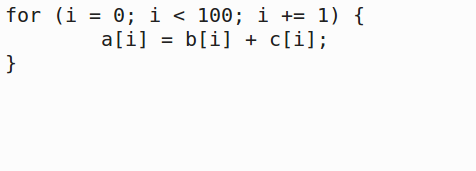
\includegraphics[width=\textwidth]{img/loop-unrolling-1.png}
    \caption{Original loop}
    \label{fig:loop-unrolling-1} 
  \end{subfigure}
  \begin{subfigure}{0.48\textwidth}
    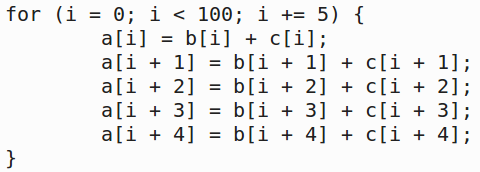
\includegraphics[width=\textwidth]{img/loop-unrolling-2.png}
    \caption{Unrolled loop}
    \label{fig:loop-unrolling-2} 
  \end{subfigure}
  \caption{By unrolling loops, instructions are made independent and the number of branches is reduced.}
  \label{fig:loop-unrolling} 
\end{figure}
Hence, to reach maximum performance for a pipelined, superscalar processor, we must find independent work. Since most programming languages do not let the programmer specify which instructions are independent of each other, compiler optimizations play a critical role in CPU utilization \cite{Boncz2005-wj}. The most widely used technique used by the compilers to address this challenge is \textit{loop unrolling}, which is used to reduce the number of branches and increase independence between instructions \cite{Wikipedia_contributors2015-zc}. As seen in Figure \ref{fig:loop-unrolling}, loop unrolling reduces the number of iterations in a loop (reduction of branches) and replaces it with multiple instances of the same instruction. If the instructions are independent, they can be processed in parallel.

\subsection{CPU Caches}
\label{sub:CPU Caches}
Since transfering data from main memory to CPU can take around $~200$ cycles, modern CPUs utilize multiple layers of on- and off-chip caches to reduce this latency. Efficient usage of caches is paramount for CPU throughput, since roughly 30\% of all instructions in a program are memory loads or stores \cite{Boncz2005-wj}. We know that IPC for DBMSes is strongly impaired by cache misses, and cache utilization is an important topic for in-memory databases \cite{Exasol2014-xh}.

The best way to tackle this challenge is to design algorithms and data structures that are \textit{cache aware} \cite{Farber2012-vh}. Designing such programs is out of the scope of this report, but it briefly boils down to two things:
\begin{itemize}
  \item \textit{Coordinate temporal and spatial locality}. Data processed together should be stored at consecutive memory addresses. Code locality is also important \cite{Neumann2011-uq}.
  \item \textit{Avoid false sharing of cache lines}. Multiple cores in a processor should not write to data belonging to the same cache entry at the same time to avoid unecessary invalidations.
\end{itemize}
\textit{Compression}, which we described in Section \ref{sec:Compression}, and \textit{vectorized execution}, which we discuss in Section \ref{sec:Loop Pipelining and Vectorized Execution}, are two techniques used to improve cache performance \cite{Larson2013-mc, Lemke2010-is}.

\textit{Prefetching} is another method used to increase cache utilization. Prefetching proactively loads data into caches such that the data is available when an instruction needs it.

Our research has identified several systems that are designed to be cache-aware, including \monetdb~\cite{Boncz2002-yj}, \mssql~\cite{Lahiri2015-mz}, and \ibm~\cite{Raman2013-em}. The developers of \exasol, the top performing database system in the TPC-H benchmark, claim that high level of data locality is one of the key factors to performance.

\subsection{Call Stack and Subroutine Invocations}
\label{sub:Call Stack and Subroutine Invocations}
\afigure{img/call-stack.png}{A call stack for a program in execution. Each stack frame contains input parameters, function return address, and local variables for a subroutine invocation. (Adapted from \cite{Wikipedia_contributors2015-od})}{fig:call-stack}{0.5}

A \textit{call stack} is commonly used in a computer program to store information and state about active subroutines \cite{Wikipedia_contributors2015-od}. Each time a subroutine is called, a \textit{stack frame} is added to the call stack that stores the input arguments, return address, and variables local to the subroutine. See Figure \ref{fig:call-stack}. The call stack can be implemented in both hardware and software, and the implementation varies between different systems. This stack-based technique implies that calling a subroutine comes at a cost; registers must be stored on the stack, and a new stack frame must be added.

Trading off time with space is usually done to address the above challenge; adding more code to improve program efficiency. \textit{Function inlining} is a technique used by compilers where the subroutine code is copied into the caller's body. This way, no new stack frame is created for the subroutine, avoiding the overhead associated with a function invocation.

\textit{Macro expansion} is another form of code generation. Macros are normally specified by the application programmer, and can be used for programmer-controlled inlining of functions or constant values. Macros can also be used to generate multiple versions of function or class definitions (templating), a technique commonly used to let a single implementation support different data types.

\section{Hardware Utilization}
\label{sec:Hardware Utilization}
In this section, we enumerate several topics, techniques, and concepts that are used to utilize the available hardware and maximize CPU throughput.

\subsection{Loop Pipelining}
\label{sub:Loop Pipelining}
The absence of loop pipelining can have dramatic effects on query performance \cite{Boncz2005-wj}. Boncz \ea~show that \mysql~uses 49 cycles per tuple because loops are not unrolled. In this system, tuples are processed one at a time with 1-2 function calls to extract the needed data from a tuple per iteration \cite{Abadi2008-dd}. Besides, evaluating a predicate is usually a small operation compared to the overhead associated with calling subroutines. In other words, most of the 49 instructions are spent managing the call stack or waiting for instruction dependencies.

To ensure proper loop pipeline behavior, compilers must be aware that pointers do not overlap, such that loop unrolling can be used \cite{Boncz2005-wj}. Operations in \monetx~are compiled with compiler hints that tell the compiler that processing a tuple is independent of the others. In standard \textit{C} compilers, this can be done by using the \texttt{\_\_restrict\_\_} pointer type.


\subsection{Vectorized Execution}
\label{sub:Vectorized Execution}
To avoid unnecessary subroutine invocation overhead and help the compiler identify which instructions are independent, \textit{vectorized execution} is normally used. Vectorized execution, or block iteration, is the technique where multiple rows are processed at the same time to avoid the overhead associated with tuple-at-a-time processing \cite{Abadi2008-dd}. Vectorized execution enables loop unrolling and memory prefetching, and minimizes cache misses \cite{Larson2013-mc}. Research performed by Abadi \ea~shows that vectorized execution in columns stores improves performance by 50\% on average.

% explain who uses it
Several systems studied our research use vectorized execution. \ibm~and \mssql~work on batches of thousands of row at a time \cite{Larson2013-mc, Raman2013-em}. \monetdb~and \monetx~use vectors instead of single values as their primary structure for storing data \cite{Boncz2005-wj, Boncz2002-yj}. Vectorized execution is also used by \cstore~and \blink~\cite{Johnson2008-cp, Stonebraker2005-qz}.

% Explain how it works.
\afigure{img/vectorized-execution.png}{\mssql~operators work on row batches. Each row batch contains thousands of rows stored as column vectors. Also, a bit vector indicates which rows that qualifies for a query. Courtesy of \cite{Larson2013-mc}.}{fig:vectorized-execution}{0.4}
In vectorized execution, blocks of values from the same column are sent to an operator for evaluation \cite{Zukowski2006-oz}. Query operators in \mssql~work on row batches, batches that contain thousands of rows stored in a column format. In addition to the column vectors, an additional \textit{qualifying rows vector} is used to indicate which rows that have been logically purged from the batch when executing a query. Figure \ref{fig:vectorized-execution} shows this structure.

Regarding the size of the vectors in vectorized execution, we have found that vectors should not be too small due to increased overhead and less parallelism, nor too big, as it should fit in CPU cache \cite{Boncz2005-wj}.

Although vectorized execution for column stores normally outperforms tuple-at-a-time query processing, there are some disadvantages by using this model. Neumann \ea~claim that vectorized execution eliminates a major strength of the iterator model, namely \textit{pipelining} \cite{Neumann2011-uq}. In this context, pipelining means the ability for an operator to pass tuples to its parent operator without copying the value. When vectorized execution is used, intermediate results have to be stored somewhere (materialized), which consumes memory bandwidth.

\subsection{Late Materialization}
\label{sub:Late Materialization}
\textit{Late materialization} is the principle of not stitching together tuples before necessary \cite{Abadi2008-dd}. Systems devoted to \textit{late materialization} work on columns for as long as possible. According to a research by Abadi \ea~\textit{late materialization} can increase performance in columns stores by 5\%-50\% depending on the query \cite{Abadi2008-dd}.

\textit{Late materialization} is advantegous because \cite{Abadi2008-dd}:
\begin{itemize}
  \item Compressed columns must be decompressed before materialization, which eliminate the benefits of working directly on compressed data. 
  \item Cache performance is better for columns than for rows, which means processing columns are more efficient. 
  \item Vectorized Execution can be used on columns only. 
  \item Early materialization might construct tuples that are discarded later in the query execution.
\end{itemize}

The \term{late materialization} principle is used by several database systems, including \ibm~\cite{Raman2013-em} and \monetdb~\cite{Boncz2002-yj}. 
\subsection{SIMD}
\label{sub:SIMD}
\afigure{img/simd.png}{SIMD execution model: In scalar mode (a): one operation produces one result. In SIMD mode (b): one operation produces multiple results. (Adapted from \cite{Willhalm2009-hu})}{fig:simd}{0.8}
% Present problem
Within a single execution context, instructions that work on multiple elements at a time can be used to increase query performance. We refer to these instructions as single input, multiple data (SIMD) instructions \cite{Wikipedia_contributors2015-ax}. As seen in Figure \ref{fig:simd}, an SIMD instruction applies the same operation to multiple operands simultaneously. SIMD processing in a database context is particularly effective if we can keep an entire processing block in the CPU registers \cite{Neumann2011-uq}, and Willhalm \ea~show that SIMD processing using a vectorized model can be up to 1.5 times faster than databases optimized for scalar execution and ILP \cite{Willhalm2009-hu}.

Our research shows that several database systems use SIMD parallelization. Systems in this category include \oracle~\cite{Lahiri2015-mz}, \blink~\cite{Barber2012-xt}, and \ibm~\cite{Raman2013-em}. A whitepaper from the developers of \exasol~says that SIMD features of modern processors must be used to reach the highest level of performance \cite{Exasol2014-xh}.

\afigure{img/oracle-simd.png}{Filter operation in \oracle~using SIMD vector processing. (Adapted from \cite{Lahiri2015-mz})}{fig:oracle-simd}{0.6}
\oracle~performs scans against the columns using instructions that work on multiple operands simultaneously \cite{Lahiri2015-mz}. As seen in Figure \ref{fig:oracle-simd}, a filter operation benefits from SIMD as multiple values are compared in parallel. \ibm~and later versions of \blink~work similarly \cite{Barber2012-xt, Raman2013-em}.

\begin{figure}
  \centering
  \begin{subfigure}{0.45\textwidth}
    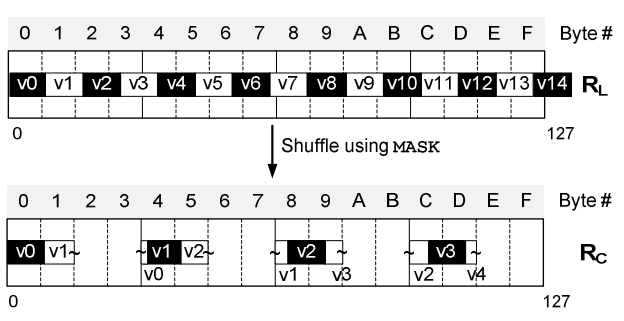
\includegraphics[width=\textwidth]{img/simd-align-1.png}
    \caption{Using a \texttt{MASK} operation to align values to data words.}
    \label{fig:simd-align-1} 
  \end{subfigure}
  \begin{subfigure}{0.45\textwidth}
    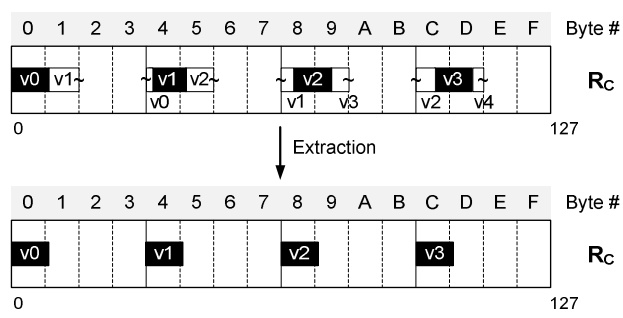
\includegraphics[width=\textwidth]{img/simd-align-2.png}
    \caption{Extracting values by bitshifting followed by masking out irrelevant bits.}
    \label{fig:simd-align-2} 
  \end{subfigure}
  \caption{Aligning a bitpacked vector for SIMD execution. (Adapted from \cite{Willhalm2009-hu})}
  \label{fig:simd-align} 
\end{figure}

Bitpacking of column values further increase SIMD performance, because more values fit within a single data word. However, since most SIMD instructions require operands to be aligned, some preprocessing steps must be applied to the column values \cite{Willhalm2009-hu}. As seen in Figure \ref{fig:simd-align}, a bitpacked vector can be prepared for an SIMD operation using mask and bitshift operations. Vectors that are already aligned with data words can be queried more efficiently since the preprocessing can be skipped.

Most literature refers to SIMD parallelization as utilizing special processor and instruction set extensions, like the Intel SSE and Intel AVX2 extension \cite{Willhalm2013-ri, Willhalm2009-hu}. However, general CPU instructions can also be used to evaluate predicates in a \textit{SIMD-like fashion}. In \blink, ordinary CPU instructions work directly on multiple values in a bitpacked column by applying a suitable mask and compare the result with a second mask containing the expected values \cite{Johnson2008-cp}. This technique is very efficient since masks for a column are calculated once per query.


\subsection{Branch Avoidance}
\label{sub:Branch Avoidance}
\ffigure{img/branch-selectivity.png}{Predicate evaluation performance for queries with different query selectivities. A \textit{branch version} and a \textit{predicated version} are tested. For the AthlonMP processor, the branch version are 2-3 times slower on queries with 40\%-60\% selectivity, while the Itanium2 processor has constant processing time. The predicated version offers constant processing time for both processors. (Adapted from \cite{Boncz2005-wj})}{fig:branch-selectivity}

We saw in Section \ref{sec:Modern CPUs and Compilers} that branches should be avoided due to the penalties of branch misprediction. Besides, branches also cause dependencies between instructions. 

The consequences of inaccurate branch prediction are studied by Neumann \ea~\cite{Neumann2011-uq}. In this research, the performance of queries with various selectivities was tested. As we can see in Figure \ref{fig:branch-selectivity}, queries with 40\%-60\% selectivity executed on an AthlonMP processor are roughly 2-3 times slower than queries with selectivities close to 0\% or 100\%. Hence, selectivity can severely affect the query performance. The Itanium2 processor does not have the same characteristic, as the Itanium architecture allows for both \textit{not taken} and \textit{taken} branches to be executed simultaneously.

Neumann \ea~also developed a branchless version (predicated version) to evaluate predicates in the queries. The branchless variant is denoted as \texttt{predicated version} in Figure \ref{fig:branch-selectivity}. For both AthlonMP and Itanium2 processors, this implementation offers constant performance for all selectivities, but is, in general, more expensive.

Branch avoidance is also important in other parts of the system, for instance when decompressing. Zukowski \ea~present a decompression algorithm that is free for \textit{if-then-else} statements \cite{Zukowski2006-oz}. By running the algorithm in two tight loops instead of one, branch misprediction is reduced, and the loops can be pipelined by a compiler.

\subsection{Macro Expansions}
\label{sub:Macro Expansions}
\afigure{img/macro-expansion.png}{Macro expansions in \monetdb. For different algorithms and data types, the \texttt{select} operator has a total of 173 implementations. (Adapted from \cite{Boncz2002-yj})}{fig:macro-expansion}{0.8}

\monetdb~uses macro expansion to reduce layers of indirection and to optimize query execution performance \cite{Boncz2002-yj}. Since operators normally are type-generic, \monetdb~has for each algorithm multiple implementations that are specific to a certain type. The implementations are generated automatically using macros, which is why they are called \textit{macro expansions}. Figure \ref{fig:macro-expansion} shows how the \texttt{select} operator is expanded into 173 implementations, depending on which algorithm and data types are queried.

The vector data structure in \ibm~is implemented using C++ templates to support multiple data types.


\subsection{Short-Circuiting}
\label{sub:Short-Circuiting}
\begin{figure}
  \centering
  \begin{subfigure}{0.45\textwidth}
    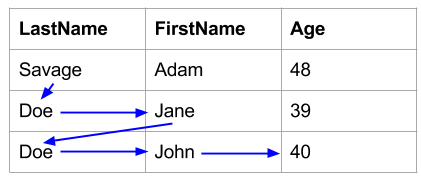
\includegraphics[width=\textwidth]{img/short-circuiting-1.png}
    \caption{Short-circuiting}
    \label{fig:short-circuiting-1} 
  \end{subfigure}
  \begin{subfigure}{0.45\textwidth}
    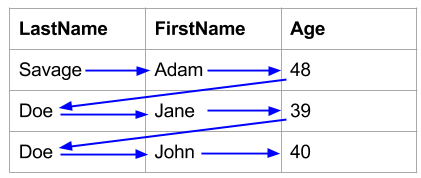
\includegraphics[width=\textwidth]{img/short-circuiting-2.png}
    \caption{No short-circuiting}
    \label{fig:short-circuiting-2} 
  \end{subfigure}
  \caption{Predicate evaluation for query \texttt{WHERE LastName='Doe' AND FirstName='John' AND Age>21}. (a) skips evaluating rest of the predicates if one predicate is false, while (b) evaluates all predicates regardless of previous results.}
  \label{fig:short-circuiting} 
\end{figure}
\textit{Short-circuiting} is referred to a special case of Boolean operator evaluation in which the next argument is not evaluated if the current argument is sufficient to determine the value of the expression \cite{Wikipedia_contributors2015-rk}. Figure \ref{fig:short-circuiting} illustrates the difference between short-circuit and non-short-circuit predicate evaluation. In short-circuiting, the scan proceeds to the next tuple as soon as one predicate is false, as opposed to the verision without short-circuiting that evaluates all predicates regardless of previous results.

Since short-circuit boolean operators are control structures and not simple arithmetic operators, there is a chance of branch misprediction. That is why \blink~does not short-circuit between tuples \cite{Raman2008-gi, Johnson2008-cp}. If a block is selected for scanning, all fields in the records are checked. According to Raman \ea, short-circuiting only improves performance on low selectivity queries \cite{Raman2008-gi}.


\section{Bitmap Indexes}
\label{sec:Bitmap Indexes}

\ffigure{img/bitmap-query.png}{Executing a query using bitmap indexes. Queries are efficiently processed using bitwise operations like \texttt{AND} and \texttt{OR}. Adapted from \cite{noauthor_undated-hp})}{fig:bitmap-query}

A \biti~is a particular structure where a bitmap represents each distinct value in a column, and all rows containing that value is set to 1. It can be used to aid predicate evaluation. A \biti~is most efficient on queries that contain multiple \texttt{WHERE} clauses since many candidate rows can be excluded using bitwise \texttt{AND} and \texttt{OR} operations, as seen in Figure \ref{fig:bitmap-query} \cite{noauthor_undated-hp}. Since bitmap indexes combine so easily, composite indexes are extraneous. 

\bd~product \qlikview~reports that it uses binary indexes for each field \cite{Qlik2011-ef}, which we believe are the same as bitmap indexes. Some database management systems also support bitmap indexes, including \oracle~\cite{noauthor_undated-hp} and \ibm~\cite{Raman2013-em}.

In general, low-cardinality columns, which is columns with few distinct values, are better suited for bitmap indexes than high-cardinality columns \cite{noauthor_undated-hp}. The reason for this is because a bitmap must be created and maintained for each unique value in the column. Besides, since these indexes are hard to maintain, they are not suited for inserts, updates, and deletes. When deciding whether to add a \biti~to a column, \oracle~recommends at least 100 rows per distinct value. 

\section{Joining}
\label{sec:Joining}
Joining is a common database operation that combines records from two or more tables. In our research, we have studied several DBMSes, and seen how their join algorithms work. For joining two tables, three main methods exist \cite{Bratbergsengen2015-ed}: 
\begin{itemize}
  \item \textit{Partition-based approach}, where records of both tables are split into groups based on the hash value of the keys. This technique is most effective on data volumes that are too large to fit in main memory.
  \item \textit{Sort-merge approach}, where both tables are sorted and then merge results by concatenating records with equal key values. This approach is most effective when one or both operands are sorted in advance.
  \item \textit{Nested loop approach}, which compares all rows in both tables.
\end{itemize}

The \textit{nested loop} approach is the most popular joining algorithm for in-memory databases \cite{Boncz2002-yj}. We therefore only discuss this method.

\subsection{Nested Loop Algorithms}
\label{sub:Nested Loop Algorithms}

% Basic nested join functionality
In its simplest form, the \textit{nested loop} method compares the join key in all rows directly using a double loop. This simple algorithm has a runtime of $O(n*m)$ where $n$ and $m$ is the size of tables A and B respectively. However, to improve performance in a \textit{nested loop} algorithm, hashmaps are commonly used. Usually, the join is performed by hashing the smaller (inner) relation first, then probe the hashmap by scanning the larger (outer) relation. 

\ffigure{img/nested-loop.png}{An example nested loop join structure. Records are first tested against a Bloom filter. If found in the filter, the join key is searched in the join structure. Records are first hashed, and then each entry in the hash table is the root of a binary tree. (Adapted from \cite{Bratbergsengen2015-ed})}{fig:nested-loop}

Kjell Bratbergsengen shows how a combination of hash tables, bloom filters, and binary trees can be used in a \textit{nested join} algorithm. In the probe phase, keys are first checked towards a Bloom filter. Bloom filters never return false negatives and is an efficient way of reducing the numbers of keys entering the join. If the key is found in the Bloom filter lookup, it is hashed and checked up against a hybrid hashmap/binary-tree structure. In this structure, each entry in the hashmap is the root node of a binary tree which are used to efficiently look up values. The join algorithm is illustrated in Figure \ref{fig:nested-loop}.

% Modifications
In the nested loop approach, one of the operands might be partitioned \cite{Bratbergsengen2015-ed}. For example, a join might be partitioned by only hashing a subset of the inner relation at a time. The entire join algorithm will then include several probe passes over the outer relation, one for each subset. Historically, this technique has been applied to ensure the whole hash structure fits in RAM. We conclude that a similar concept can be applied to CPU caches and that the join algorithm might benefit from partitioning the inner relation such that each subset fits in the CPU cache.

We see that several DBMSes in this research use a \textit{nested loop} join variant with Bloom filters, including \oracle~\cite{Lahiri2015-mz}, \ibm~\cite{Raman2013-em} and \blink~\cite{Raman2008-gi}. Barber \ea~explains how Bloom filters are effective in eliminating non-matching join outers before they enter the join \cite{Barber2014-ey}.

Our research has shown that one of the key design goals for efficient joining using the \textit{nested loop} approach with hashmaps, is to keep the hash tables collision free \cite{Raman2008-gi, Raman2013-em}. One way to ensure this is to use the dictionary keys in \de~as a perfect hashing function. If a table is joined on several keys, a minimal perfect hash can be calculated.

Regarding implementation, it is important that the algorithm and the hash table are \textit{cache-aware}. One way to improve cache performance in a \textit{nested loop} join, is to use linear probing instead of open-chain addressing for the hashmap \cite{Raman2008-gi}. Open-chain addressing should only be used for overflow buckets.

\section{Database Statistics}
\label{sec:Database Statistics}
\term{Database Statistics} are commonly used by a query optimizer to make better decisions about creating efficient execution plans. These statistics may the include number of records, selectivity, column cardinality, value distribution, and more. In our case, \term{Database Statistics} can be used to prune horizontal partions based on the column minimum and maximum values. This technique exploits clustering in the columns, especially when the columns are sorted, or partially sorted, like timestamps. \oracle~\cite{Lahiri2015-mz}, \ibm~\cite{Raman2013-em}, \vertica~\cite{Lamb2012-kg}, \monetx~\cite{Boncz2005-wj}, \mssql~\cite{Larson2013-mc}, and \exasol~\cite{Exasol2014-xh} store partition metadata for quick data pruning.

Most database systems keep the statistics stored together with the table. However, other schemes exist. \ibm~uses a synopsis table to keep track of all column pages (partitions), including minimum and maximum values. This way, irrelevant pages can easily be skipped \cite{Raman2013-em}.

We have previously discussed how a partition dictionary can be checked for a key's existence before scanning an entire block. If a key is not present in the dictionary, the partition can be skipped. We consider this technique as a part of utilizing \term{Database Statistics} to improve performance.

It can sometimes be useful to know a column's value distribution. For instance, the frequency partitioning in \blink~and \ibm~uses the columns' value distributions when determining how to partition the data \cite{Raman2008-gi, Raman2013-em}. The query optimizer in \mssql~also uses the value distributions when creating execution plans \cite{Larson2013-mc}. Value distributions are usually determined by creating histograms, and to make these histograms, random sampling can be used. In \mssql, two techniques are used: One is truly random, where values are picked across the whole column, and one is a grouped version, where a random sample range is picked.

\section{Testing OLAP Databases}
\label{sec:Testing OLAP Databases}
The TPC-H benchmark is commonly used to test analytical workloads. The benchmark is made for decision support workloads and consists of a suite of business oriented ad-hoc queries \cite{Transaction_Processing_Performance_Council_TPC2014-ux}. The benchmark has 22 complex read-only queries, which are both memory and CPU bound \cite{Boncz2005-wj}, and two update queries for data refresh. The TPC-H specification says the benchmark illustrates a decision support system that:
\begin{itemize}
  \item Examine large volumes of data.
  \item Execute queries with a high degree of complexity.
  \item Give answers to critical business questions.
\end{itemize}

\afigure{img/tpc-h.png}{The TPC-H schema. (Adapted from \cite{Transaction_Processing_Performance_Council_TPC2014-ux})}{fig:tpc-h}{0.8}
The schema for the TPC-H benchmark consists of eight separate tables, as seen in Figure \ref{fig:tpc-h}. The table columns have a variety of different data types, including integers, floating points, variable and fixed width strings, identifiers, and booleans. 

\afigure{img/tpc-h-population.png}{TPC-H database size and cardinalities. (Adapted from \cite{Transaction_Processing_Performance_Council_TPC2014-ux})}{fig:tpc-h-population}{0.8}
Figure \ref{fig:tpc-h-population} shows the minimum population for the TPC-H benchmark, which is a database of 10,000 suppliers and roughly 6 million line-items (items per order). The minimum population corresponds to roughly 1 GB. To test larger data sizes, a scaling factor is commonly applied to increase the size of the dataset. According to the specification, data in the tables should be uniformly distributed.

The TPC-H benchmark tests uniformly distributed data, but, in reality, it is quite common that data is skewed. For instance, a retailer might expect that 99\% of the sales are performed on weekdays, and around 40\% of the total sales for a year is done around Christmas \cite{Raman2008-gi}. Tests on data with non-uniform distributions should be performed to see how the algorithms and data structures in the database handle outliers. Data skew can be modelled with a \term{Zipfian} distribution \cite{Holloway2008-rr}. 


